\section*{Überblick}

\begin{figure}[htb]
\begin{center}
%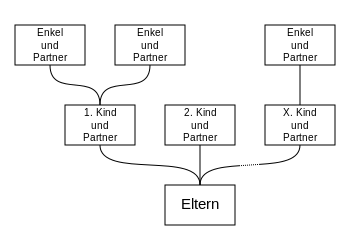
\includegraphics[width=.7\textwidth]{../fig/stammbaum.png}
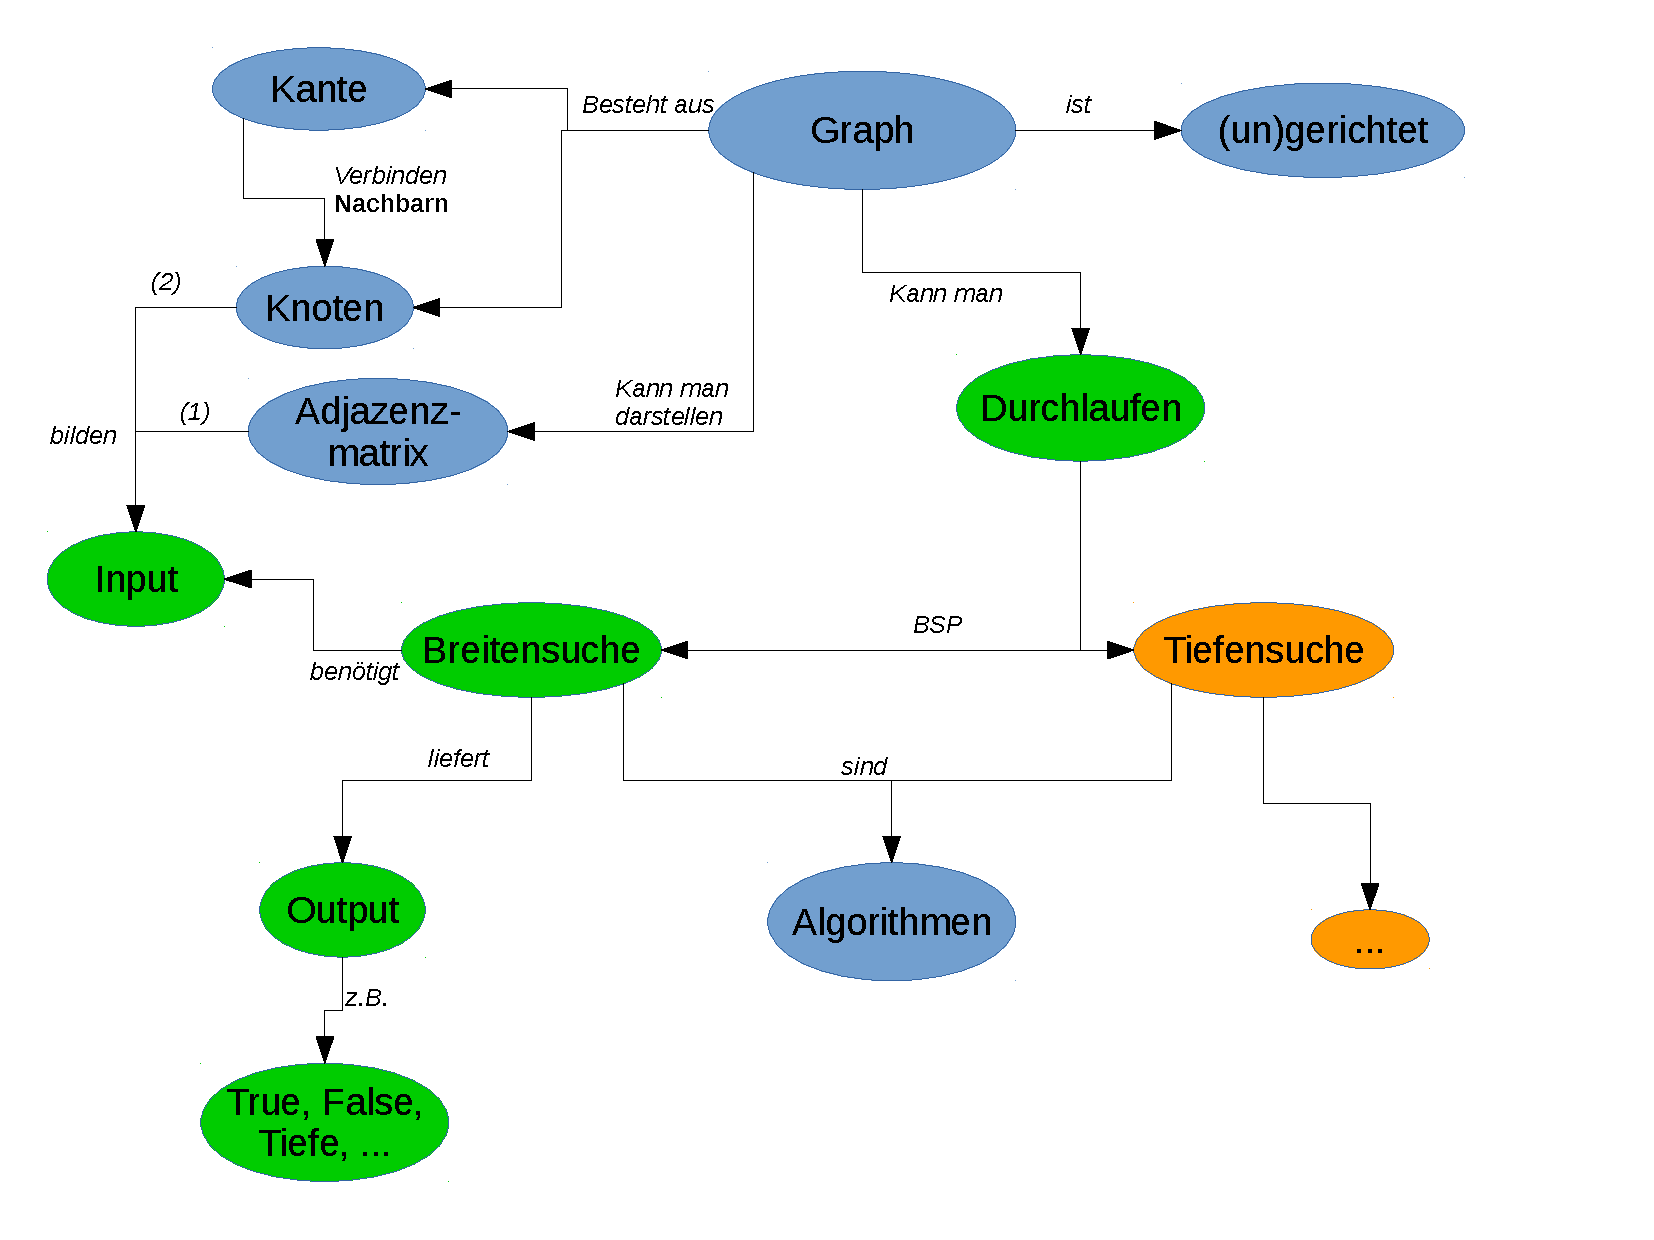
\includegraphics[width=.99\textwidth]{../cmap/bsuche_cmap.pdf}
\caption{Concept-Map zum Thema Breitensuche.
Blaue Konzepte bilden das Vorwissen ab. 
Grüne Konzepte werden in dieser Arbeit eingeführt und behandelt. 
Orangene Konzepte bilden einen Ausblick auf Konzepte, welche im Rahmen dieser Arbeit nicht mehr behandelt werden. 
}
\label{fig:cmap2}
\end{center}
\end{figure}


Den Begriff Graph haben Sie schon einmal gehört. Mit einem Graphen kann man verschiedene Objekte mit einander verbinden. 
Eine interessante Frage ist immer über wie viele Verbindung zwei Objekte mit einander verknüpft sind. 
Wir möchten nun mit diesem Kapitel überlegen, wie man einen Graphen durchsuchen kann.
Ein Beispiel für einen solchen Algorithmus ist die Breitensuche. 
Ziel ist es, dass Sie den Algorithmus verstehen und anwenden können. 

Der Aufbau dieses Kapitels ist so gehalten, dass Sie im ersten Abschnitt nochmal die Grundlagen zu Graphen wiederholen und festigen. 
Dabei geht es vor allem um verschiedene Darstellungen von Graphen und das Konzept von Nachbarn.


%TODO sehr kurz vielleicht besser formulieren?
Im zweiten Teil werden Sie dann die Breitensuche an sich behandeln und auf verschiedene Probleme anwenden.

In der folgenden Concept-Map (s. Abb.~\ref{fig:cmap2} können Sie die verschiedenen Konzepte und ihren Zusammenhang für das folgende Kapitel überblicken.

